\documentclass[tikz,border=4pt]{standalone}
\usepackage{amsmath}
\usepackage{times}
\usetikzlibrary{arrows.meta,positioning,shapes.geometric,calc}
\begin{document}
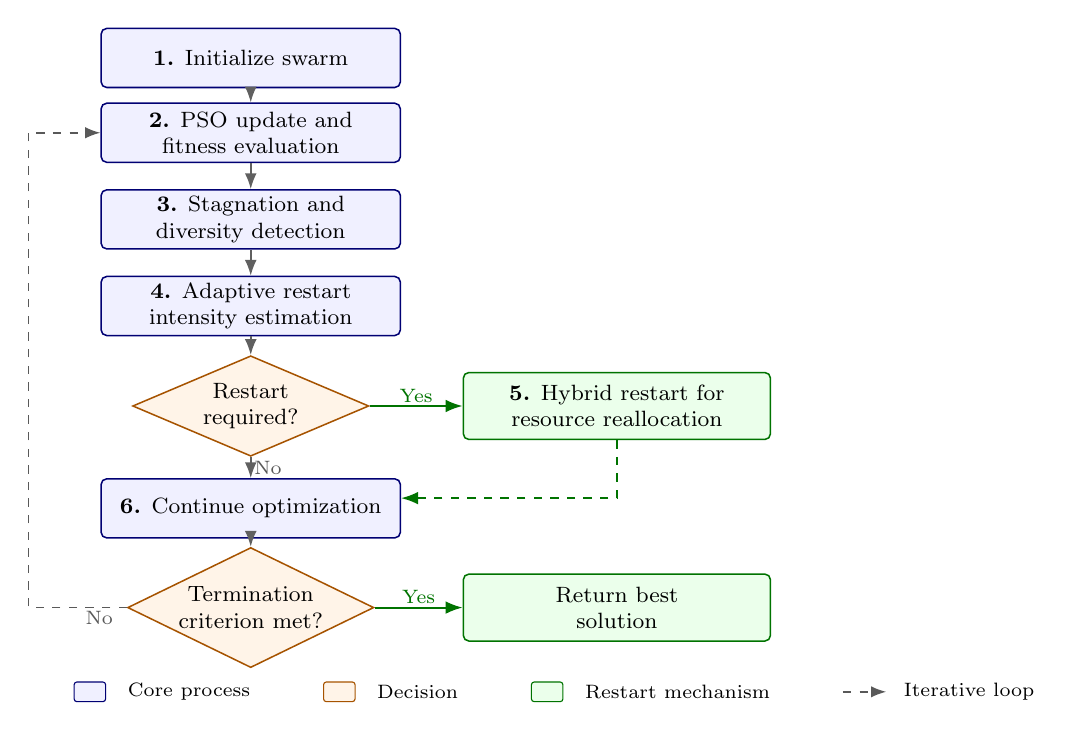
\begin{tikzpicture}[
    font=\footnotesize,
    >=Latex,
    process/.style={
        rectangle,
        rounded corners=2pt,
        draw=blue!45!black,
        fill=blue!6,
        line width=0.55pt,
        minimum width=38mm,
        minimum height=7.5mm,
        align=center,
        inner xsep=3pt,
        inner ysep=2pt
    },
    decision/.style={
        diamond,
        aspect=2.05,
        draw=orange!65!black,
        fill=orange!9,
        line width=0.55pt,
        minimum width=30mm,
        minimum height=12mm,
        align=center,
        inner sep=1pt
    },
    restart/.style={
        rectangle,
        rounded corners=2pt,
        draw=green!45!black,
        fill=green!8,
        line width=0.55pt,
        minimum width=39mm,
        minimum height=8.5mm,
        align=center,
        inner xsep=3pt,
        inner ysep=2pt
    },
    flow/.style={->, line width=0.6pt, draw=gray!75!black},
    yesflow/.style={->, line width=0.7pt, draw=green!45!black},
    loop/.style={->, dashed, line width=0.55pt, draw=gray!70!black},
    note/.style={font=\scriptsize, inner sep=1pt},
    legendbox/.style={
        rectangle,
        rounded corners=1pt,
        minimum width=4mm,
        minimum height=2.5mm,
        inner sep=0pt,
        line width=0.4pt
    }
]

\node[process] (init) at (0,0) {\textbf{1.} Initialize swarm};
\node[process] (update) at (0,-0.95) {\textbf{2.} PSO update and\\fitness evaluation};
\node[process] (detect) at (0,-2.05) {\textbf{3.} Stagnation and\\diversity detection};
\node[process] (intensity) at (0,-3.15) {\textbf{4.} Adaptive restart\\intensity estimation};
\node[decision] (restartq) at (0,-4.42) {Restart\\required?};
\node[process] (continue) at (0,-5.72) {\textbf{6.} Continue optimization};
\node[decision] (termq) at (0,-6.98) {Termination\\criterion met?};

\node[restart] (hybrid) at (4.65,-4.42) {\textbf{5.} Hybrid restart for\\resource reallocation};
\node[restart] (return) at (4.65,-6.98) {Return best\\solution};

\draw[flow] (init) -- (update);
\draw[flow] (update) -- (detect);
\draw[flow] (detect) -- (intensity);
\draw[flow] (intensity) -- (restartq);
\draw[flow] (restartq) -- node[note, right, text=gray!70!black] {No} (continue);
\draw[flow] (continue) -- (termq);

\draw[yesflow] (restartq.east) -- node[note, above, text=green!45!black] {Yes} (hybrid.west);
\draw[yesflow, dashed] (hybrid.south) |- ($(continue.east)+(0,0.13)$);
\draw[yesflow] (termq.east) -- node[note, above, text=green!45!black] {Yes} (return.west);

\draw[loop] (termq.west) -- ++(-1.25,0)
    node[note, below, pos=0.28, text=gray!70!black] {No} |- (update.west);

\coordinate (legendbase) at (-2.25,-8.05);
\node[legendbox, draw=blue!45!black, fill=blue!6, anchor=west] (l1) at (legendbase) {};
\node[anchor=west, right=1.5mm of l1] (l1t) {\scriptsize Core process};
\node[legendbox, draw=orange!65!black, fill=orange!9, anchor=west, right=8mm of l1t] (l2) {};
\node[anchor=west, right=1.5mm of l2] (l2t) {\scriptsize Decision};
\node[legendbox, draw=green!45!black, fill=green!8, anchor=west, right=8mm of l2t] (l3) {};
\node[anchor=west, right=1.5mm of l3] (l3t) {\scriptsize Restart mechanism};
\draw[loop] ($(l3t.east)+(0.8,0)$) -- ++(0.55,0);
\node[anchor=west] at ($(l3t.east)+(1.45,0)$) {\scriptsize Iterative loop};

\end{tikzpicture}
\end{document}
